\documentclass[letterpaper, 10pt]{article}
\usepackage[utf8]{inputenc}
\usepackage{amsmath}
\usepackage{amsfonts}
\usepackage{amssymb}
\usepackage[letterpaper, margin=1in]{geometry}

\usepackage{pgfplots}
\usepackage{xcolor}
\usepackage{listings}
\usepackage{layouts}
\usepackage[section]{placeins}
\lstset{ 
	% language=Python,                	% choose the language of the code
	basicstyle=\ttfamily\footnotesize, 	% the size of the fonts that are used for the code
	numbers=left,                   	% where to put the line-numbers
	numberstyle=\ttfamily\footnotesize, % the size of the fonts that are used for the line-numbers
	stepnumber=1,                   	% the step between two line-numbers. If it is 1 each line will be numbered
	numbersep=5pt,                  	% how far the line-numbers are from the code
	backgroundcolor=\color{white}, 		% choose the background color. You must add \usepackage{color}
	showspaces=false,               	% show spaces adding particular underscores
	showstringspaces=false,         	% underline spaces within strings
	showtabs=false,                 	% show tabs within strings adding particular underscores
	frame=single,           			% adds a frame around the code
	tabsize=4,          				% sets default tabsize to 4 spaces
	captionpos=t,           			% sets the caption-position to bottom
	breaklines=true,        			% sets automatic line breaking
	breakatwhitespace=false,    		% sets if automatic breaks should only happen at whitespace
	escapeinside={\%*}{*)}          	% if you want to add a comment within your code
	% prebreak=\raisebox{0ex}[0ex][0ex]{\ensuremath{\hookleftarrow}})
}

\graphicspath{{./figures/}}

% \pagenumbering{gobble}

\begin{document}

\section*{Problem 1}
\begin{figure}[h]
	\centering
    \begin{minipage}{0.32\textwidth}
        \centering
        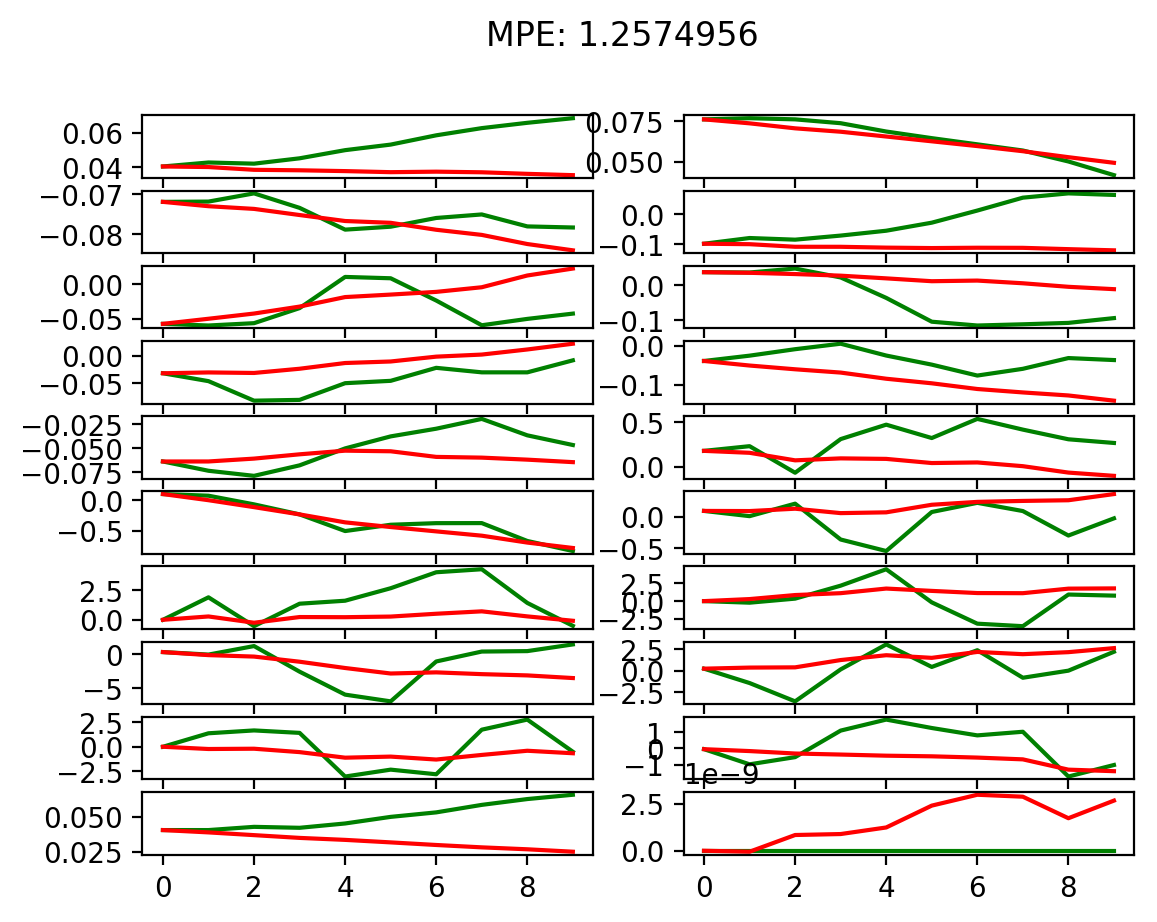
\includegraphics[width=\textwidth]{itr_0_predictions_n5_arch2x250}
        \caption{2 hidden layers, 250 units, 5 iterations}
    \end{minipage} \hfill
    \begin{minipage}{0.32\textwidth}
        \centering
        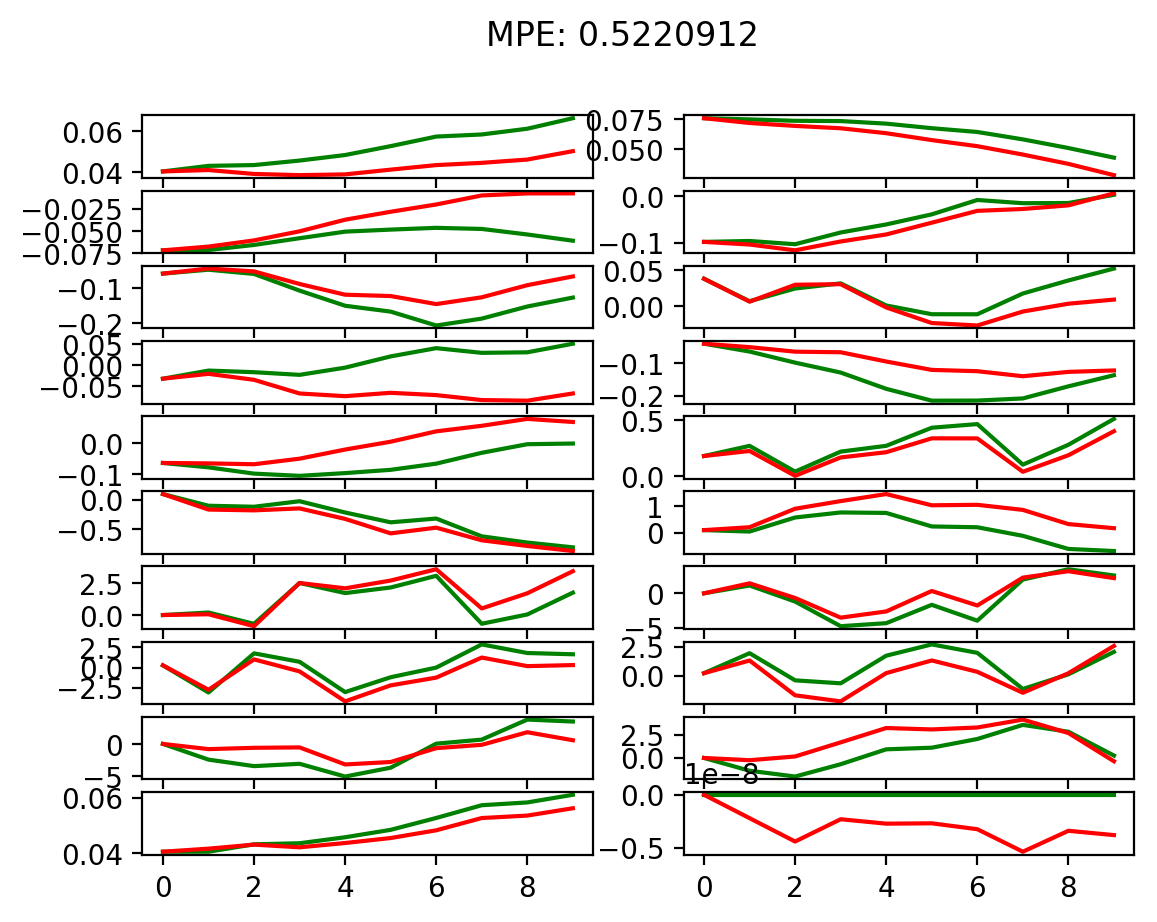
\includegraphics[width=\textwidth]{itr_0_predictions_n500_arch1x32}
        \caption{1 hidden layer, 32 units, 500 iterations}
    \end{minipage} \hfill
    \begin{minipage}{0.32\textwidth}
        \centering
        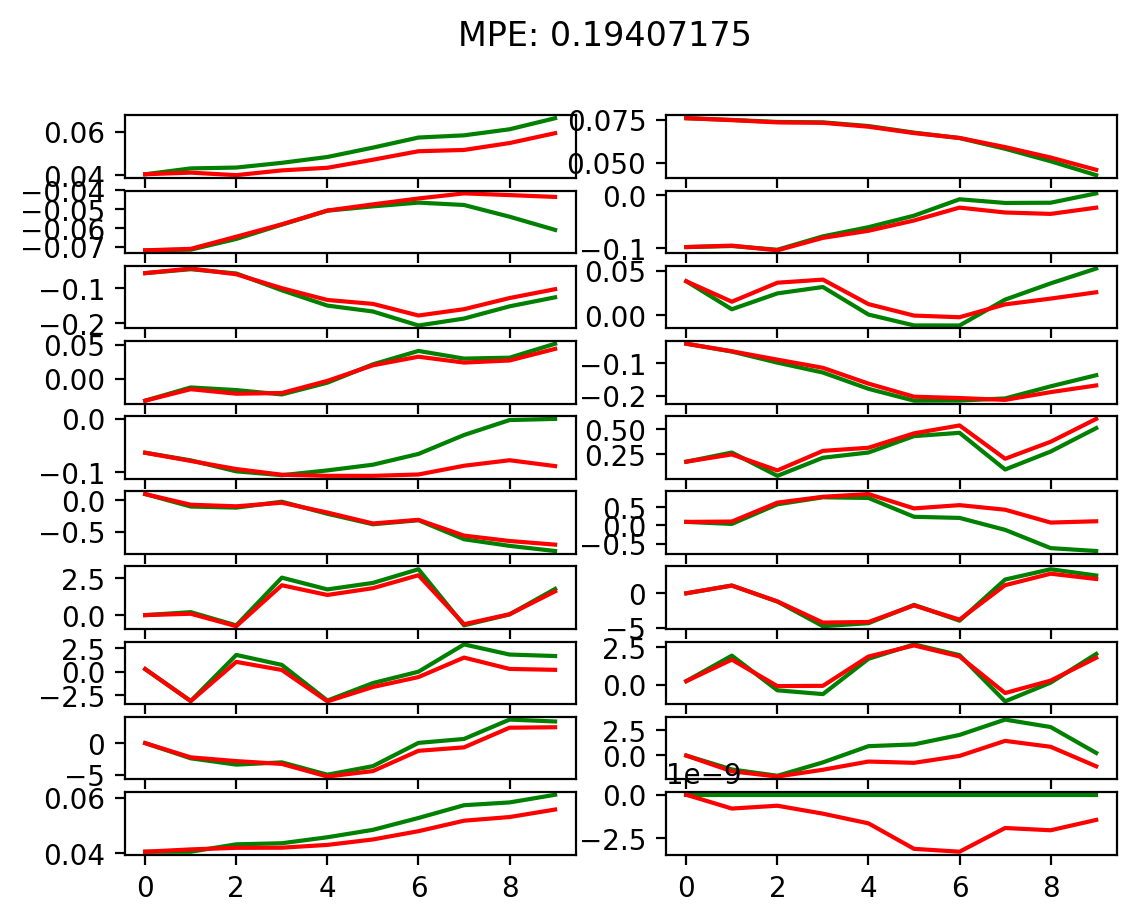
\includegraphics[width=\textwidth]{itr_0_predictions_n500_arch2x250}
        \caption{2 hidden layers, 250 units, 500 iterations}
    \end{minipage}
\end{figure}

In figure 1, we can see the performance of the neural network architecture with 2 layers, each with
250 hidden units and 5 iterations of training. This model performed the worst with the highest MPE and 
the clearest deviations from the ground truth. This was likely because despite having a very expressive
architecture, it was only trained for 5 iterations, which was not enough training time for the model.

In figure 2, we can see the performance of neural network with only a single layer with 32 hidden units. This
model performed the second best and had a much lower MPE than the previous model likely due to the much longer
training time of 500 iterations (compared to 5). However, because this was a smaller network that was not as
expressive, which may have limited its performance. 

In figure 3, we can see the best performing model. This model had both long training time (500 iterations) 
and was very large (2 layers, 250 hidden units), so the dynamics model was extremely expressive and trained 
until it was quite accurate. This model had the lowest MPE as well. 

\section*{Problem 2}

\begin{figure}[h]
	\centering
	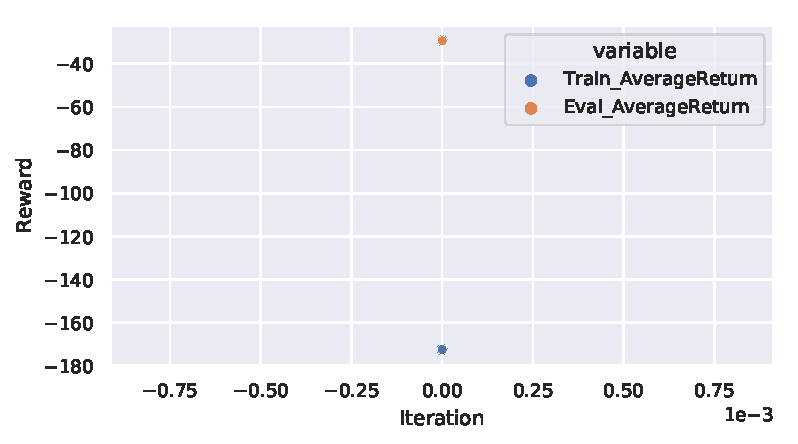
\includegraphics{q2.pdf}
	\caption{As expected, the \texttt{Eval\_AverageReturn} is much higher than the \texttt{Train\_AverageReturn}.}
\end{figure}

\section*{Problem 3}
\begin{figure}[h]
	\centering
    \begin{minipage}{0.32\textwidth}
        \centering
        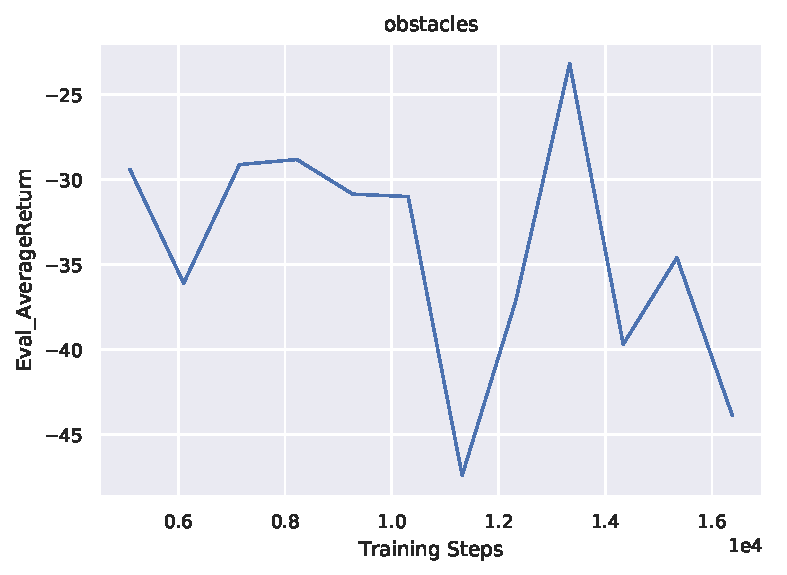
\includegraphics[width=\textwidth]{q3_obstacles.pdf}
        \caption{Obstacles Average Return}
    \end{minipage} \hfill
    \begin{minipage}{0.32\textwidth}
        \centering
        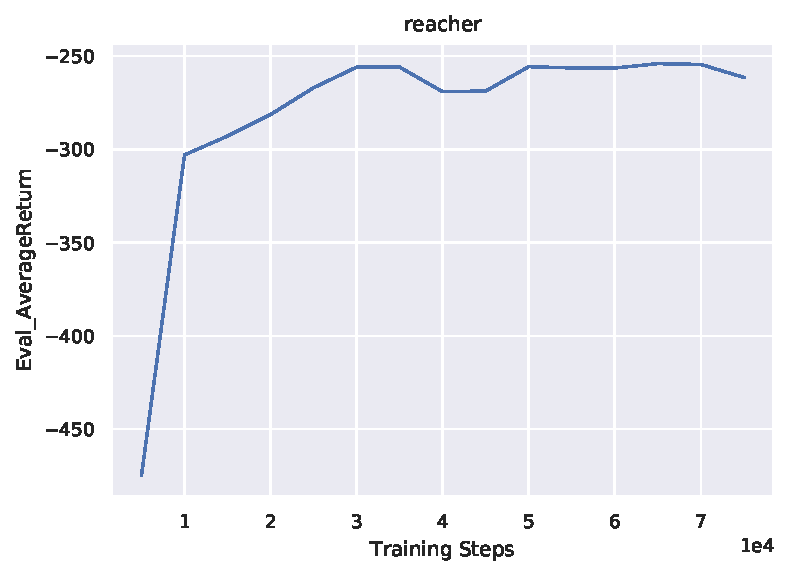
\includegraphics[width=\textwidth]{q3_reacher.pdf}
        \caption{Reacher Average Return}
    \end{minipage} \hfill
    \begin{minipage}{0.32\textwidth}
        \centering
        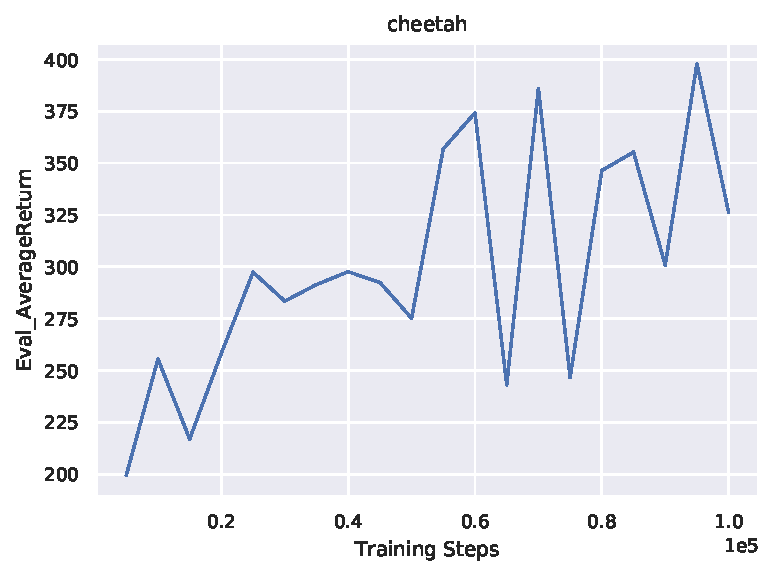
\includegraphics[width=\textwidth]{q3_cheetah.pdf}
        \caption{Cheetah Average Return}
    \end{minipage}
\end{figure}

\section*{Problem 4}
\begin{figure}[h]
	\centering
	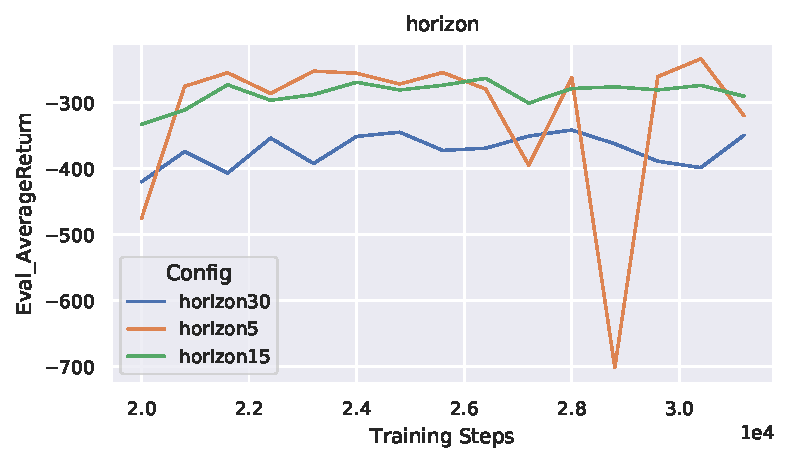
\includegraphics{q4_horizon.pdf}
	\caption{The shorter planning horizons (5 or 15) have similar performance, hovering around the same value. 
			The longer planning horizon (30) has noticably lower performance, likely due to the accumulation
			of error in the dynamics model. The use of MPC may be the reason behind the little difference 
			between 5 and 15 timestep planning horizon, since only the first action in each sequence is
			executed.}
\end{figure}

\begin{figure}[h]
	\centering
	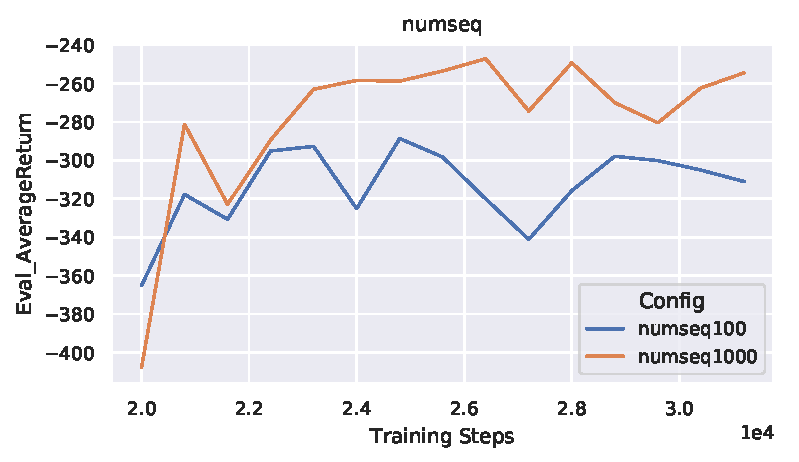
\includegraphics{q4_numseq.pdf}
	\caption{Having a higher number of candidate action sequences performs better than a lower number
			of action sequences. With a higher number of candidate sequences, the random shooting method
			is more likely to produce a high return action sequence.}
\end{figure}

\begin{figure}[h]
	\centering
	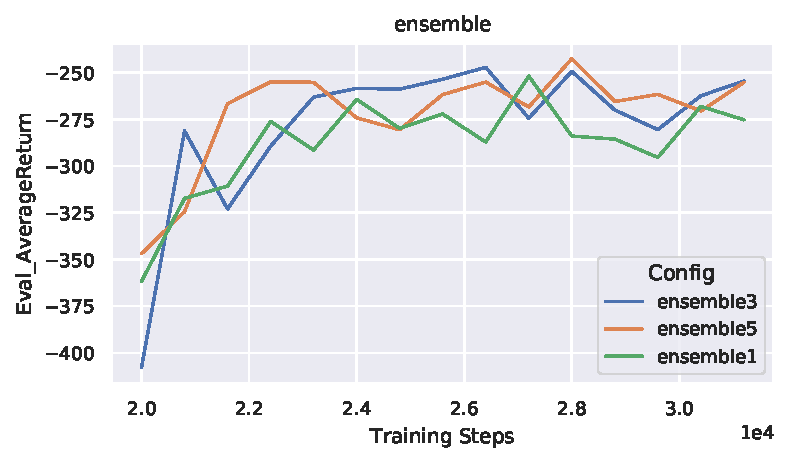
\includegraphics{q4_ensemble.pdf}
	\caption{Ensemble size does not appear to have noticable effect on the performance of the model. }
\end{figure}
\end{document}